% World side: latent-action world models drop the action labels, but the
% inverse dynamics model reads the future frame, so the bottleneck can carry it.
\documentclass[border=4pt]{standalone}
\usepackage{tikz}
\usetikzlibrary{arrows.meta, positioning, calc, backgrounds}

\definecolor{otblue}{HTML}{4472C4}
\definecolor{otred}{HTML}{C8243C}
\definecolor{otgray}{HTML}{5A5A5A}
\definecolor{otnavy}{HTML}{1F3864}

\begin{document}
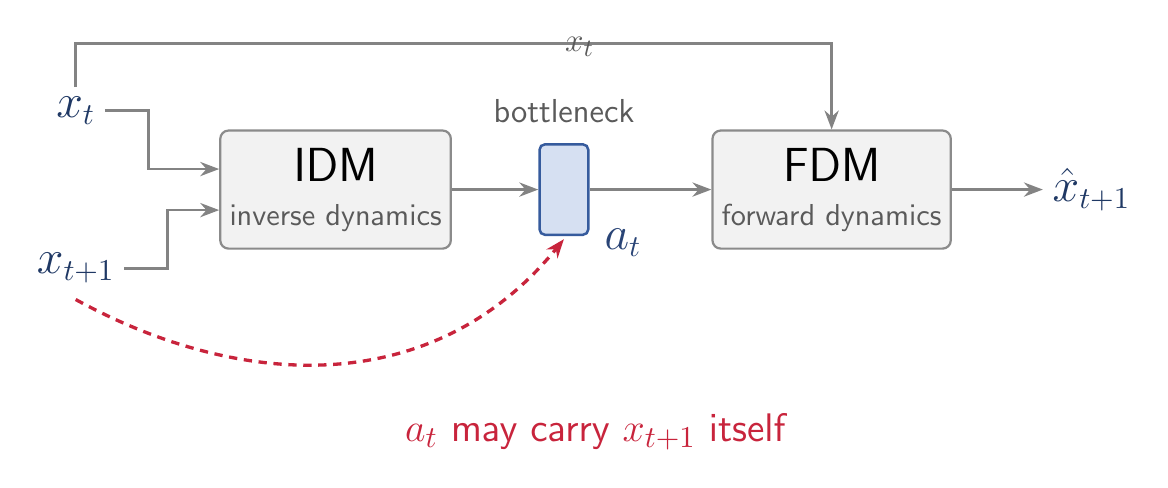
\begin{tikzpicture}[
    font=\sffamily\fontsize{16}{18}\selectfont,
    >={Stealth[length=2.4mm]},
    blk/.style={draw=otgray!70, fill=otgray!8, rounded corners=3pt,
                minimum width=1.9cm, minimum height=1.15cm, line width=0.8pt},
    lbl/.style={font=\sffamily\fontsize{16}{18}\selectfont, text=otnavy},
    flow/.style={draw=otgray!75, line width=1pt, ->},
  ]

  \node[lbl] (xt)  at (0,2.55) {$x_t$};
  \node[lbl] (xt2) at (0,0.55) {$x_{t+1}$};

  \node[blk, minimum width=2.8cm, minimum height=1.5cm, align=center] (idm) at (3.3,1.55)
    {IDM\\[-2pt]{\fontsize{10.5}{11.5}\selectfont\color{otgray}inverse dynamics}};
  \node[draw=otblue!80!black, fill=otblue!22, line width=0.9pt, rounded corners=2pt,
        minimum width=0.62cm, minimum height=1.15cm] (z) at (6.2,1.55) {};
  \node[lbl, text=otblue!60!black] at (6.95,0.88) {$a_t$};
  \node[font=\sffamily\fontsize{13}{15}\selectfont, text=otgray] at (6.2,2.55) {bottleneck};

  \node[blk, minimum width=2.8cm, minimum height=1.5cm, align=center] (fdm) at (9.6,1.55)
    {FDM\\[-2pt]{\fontsize{10.5}{11.5}\selectfont\color{otgray}forward dynamics}};
  \node[lbl] (out) at (12.9,1.55) {$\hat{x}_{t+1}$};

  \draw[flow] (xt.east)  -- ++(0.55,0) |- (idm.170);
  \draw[flow] (xt2.east) -- ++(0.55,0) |- (idm.190);
  \draw[flow] (idm.east) -- (z.west);
  \draw[flow] (z.east)   -- (fdm.west);
  \draw[flow] (fdm.east) -- (out.west);

  % x_t also goes straight to the forward model
  \draw[flow] (xt.north) -- ++(0,0.55) -| (fdm.north);
  \node[font=\sffamily\fontsize{13}{15}\selectfont, text=otgray, anchor=south]
    at (6.4,3.12) {$x_t$};

  % the leak: the future frame can ride straight into the bottleneck
  \draw[otred, line width=1.2pt, dash pattern=on 3pt off 2.4pt, ->]
    ($(xt2.south)+(0,-0.08)$) .. controls (2.2,-1.05) and (4.6,-1.05) .. (6.2,0.92);
  \node[font=\sffamily\fontsize{15}{17}\selectfont, text=otred, anchor=north]
    at (6.6,-1.18) {$a_t$ may carry $x_{t+1}$ itself};
\end{tikzpicture}
\end{document}
